\documentclass[letterpaper]{article}
\usepackage[submission]{aaai2027}
\usepackage[hyphens]{url}
\usepackage{graphicx}
\urlstyle{rm}
\def\UrlFont{\rm}
\usepackage{natbib}
\usepackage{caption}
\usepackage{booktabs}
\usepackage{amsmath}
\frenchspacing

\pdfinfo{
/TemplateVersion (2027.1)
}

\setcounter{secnumdepth}{0}
\newcommand{\PublicSkillCount}{79,141}
\newcommand{\PublicTaskCount}{73}
\newcommand{\PublicVariantCount}{219}
\newcommand{\PublicGoldCount}{182}
\newcommand{\WordEnHit}{37.0\%}
\newcommand{\WordEnRecall}{46.8\%}
\newcommand{\WordEnNdcg}{0.370}
\newcommand{\WordZhHit}{8.2\%}
\newcommand{\WordZhRecall}{17.7\%}
\newcommand{\WordZhNdcg}{0.116}
\newcommand{\WordInstHit}{8.2\%}
\newcommand{\WordInstRecall}{17.7\%}
\newcommand{\WordInstNdcg}{0.114}
\newcommand{\WordLatency}{5.7}
\newcommand{\BmEnHit}{46.6\%}
\newcommand{\BmEnRecall}{46.0\%}
\newcommand{\BmEnNdcg}{0.391}
\newcommand{\BmZhHit}{19.2\%}
\newcommand{\BmZhRecall}{21.7\%}
\newcommand{\BmZhNdcg}{0.168}
\newcommand{\BmInstHit}{12.3\%}
\newcommand{\BmInstRecall}{17.1\%}
\newcommand{\BmInstNdcg}{0.127}
\newcommand{\BmLatency}{5.6}
\newcommand{\CharEnHit}{49.3\%}
\newcommand{\CharEnRecall}{50.1\%}
\newcommand{\CharEnNdcg}{0.432}
\newcommand{\CharZhHit}{21.9\%}
\newcommand{\CharZhRecall}{31.4\%}
\newcommand{\CharZhNdcg}{0.235}
\newcommand{\CharInstHit}{24.7\%}
\newcommand{\CharInstRecall}{29.4\%}
\newcommand{\CharInstNdcg}{0.236}
\newcommand{\CharLatency}{14.8}
\newcommand{\EfiveEnHit}{13.7\%}
\newcommand{\EfiveEnRecall}{15.5\%}
\newcommand{\EfiveEnNdcg}{0.119}
\newcommand{\EfiveZhHit}{0.0\%}
\newcommand{\EfiveZhRecall}{0.0\%}
\newcommand{\EfiveZhNdcg}{0.000}
\newcommand{\EfiveInstHit}{0.0\%}
\newcommand{\EfiveInstRecall}{0.0\%}
\newcommand{\EfiveInstNdcg}{0.000}
\newcommand{\EfiveLatency}{12.0}
\newcommand{\SrEnHit}{45.2\%}
\newcommand{\SrEnRecall}{50.5\%}
\newcommand{\SrEnNdcg}{0.412}
\newcommand{\SrZhHit}{41.1\%}
\newcommand{\SrZhRecall}{43.8\%}
\newcommand{\SrZhNdcg}{0.366}
\newcommand{\SrInstHit}{26.0\%}
\newcommand{\SrInstRecall}{38.9\%}
\newcommand{\SrInstNdcg}{0.298}
\newcommand{\SrLatency}{140.8}
\newcommand{\FusionEnHit}{49.3\%}
\newcommand{\FusionEnRecall}{54.9\%}
\newcommand{\FusionEnNdcg}{0.456}
\newcommand{\FusionZhHit}{42.5\%}
\newcommand{\FusionZhRecall}{46.0\%}
\newcommand{\FusionZhNdcg}{0.375}
\newcommand{\FusionInstHit}{39.7\%}
\newcommand{\FusionInstRecall}{42.1\%}
\newcommand{\FusionInstNdcg}{0.353}
\newcommand{\FusionLatency}{155.6}
\newcommand{\SparseLatencyRange}{5.6--14.8}
\newcommand{\SrVsCharZhSignificance}{$p=0.013$, exact McNemar, 21 gains vs. 7 losses}
\newcommand{\SrVsCharInstSignificance}{$p=1.000$, exact McNemar, 14 gains vs. 13 losses}


\title{Bilingual Skill Routing at 80K Scale: Domain Adaptation and Instruction Prefixes}
\author{Anonymous Submission}
\affiliations{}

\begin{document}
\maketitle

\begin{abstract}
Agent skills are reusable instruction packages selected before an agent loads
their full procedures.  This progressive-disclosure design makes routing a
high-leverage decision, but current skill-routing benchmarks are
English-centric.
We introduce a bilingual evaluation that adds faithful Chinese translations
and fixed bilingual-instruction variants to \PublicTaskCount{} public
SkillRouter tasks while
preserving their expert skill labels.  We retrieve from \PublicSkillCount{}
hard-tier skills using word TF--IDF, BM25, character TF--IDF,
multilingual-E5, a skill-domain encoder, and reciprocal-rank fusion.  The
domain encoder obtains \SrZhHit{} Hit@1 on Chinese queries versus
\WordZhHit{} for word TF--IDF.  Complementing it with character evidence
reaches \FusionZhHit{} Hit@1 in Chinese and \FusionInstHit{} when a fixed
bilingual instruction prefixes the Chinese task.  The results expose
two practical asymmetries: domain adaptation matters more than generic
multilinguality, and a repeated bilingual instruction can reduce dense
retrieval quality even when it helps lexical fusion.  All evaluations are
local and reproducible; we release query variants, checksums, code, confidence
intervals, rankings, and latency measurements.
\end{abstract}

\section{Introduction}

Agent hosts increasingly package reusable behavior as \emph{skills}: folders
containing a short name and description, a full instruction file, and optional
scripts or references.  The Agent Skills specification formalizes this
progressive-disclosure pattern: metadata is always visible, instructions are
loaded after activation, and larger resources are read only when needed
\cite{agentskills2025spec,zhang2025equipping}.  This design saves context, but
it also creates an upstream bottleneck.  If the router surfaces the wrong
skill, a capable downstream model receives the wrong procedure.

Recent work establishes that the bottleneck is real.  SkillsBench measures
whether skills improve task execution \cite{li2026skillsbench}, while
SkillRouter evaluates retrieval from roughly 80K skills and finds that full
skill text provides important evidence in highly overlapping pools
\cite{zheng2026skillrouter}.  These benchmarks, however, are distributed as
English data.  A common deployment setting is bilingual: a user states intent in Chinese
while the registry metadata remains entirely English.  Hosts may also prepend
a bilingual routing instruction to a non-English request.  This cross-lingual
mismatch occurs \emph{before} tool execution, so evidence about multilingual
function calling \cite{guo2024ctooleval,luo2026lost} does not tell us whether
the correct skill is discovered.

We study this problem by constructing
Chinese and instruction-prefixed Chinese variants of the public SkillRouter
hard-tier tasks
and retrieve from \PublicSkillCount{} candidates.  The variants preserve the
original gold skills and all executable constraints.  We compare sparse
lexical methods, a compact generic multilingual encoder, the released
skill-domain encoder, and rank fusion.

Our contributions are:
\begin{itemize}
  \item a \PublicTaskCount{}-task, \PublicVariantCount{}-query bilingual
  extension of a public 79K-skill benchmark, with English, Chinese, and
  fixed bilingual-instruction variants tied to the same expert labels;
  \item an evaluation of TF--IDF, BM25, character retrieval, generic
  multilingual-E5, a skill-domain encoder, and fusion under Hit@1, Hit@5,
  recall@10, NDCG@10, confidence intervals, paired tests, indexing cost, and
  query latency; and
  \item a task-level analysis showing when domain adaptation transfers across
  language and how a fixed bilingual instruction changes sparse, dense, and
  fused retrieval differently.
\end{itemize}

\section{Related Work}

\paragraph{Skills and large registries.}
The Agent Skills specification defines short routing metadata and delayed
instruction loading \cite{agentskills2025spec}.  SkillsBench evaluates the
downstream value of modular procedures \cite{li2026skillsbench}.  SkillRouter
directly studies large-pool retrieval and introduces a learned
retrieve--rerank pipeline over full skill text \cite{zheng2026skillrouter}.
Our work keeps SkillRouter's hard candidate pool and expert labels, but asks a
different question: how robust is \emph{metadata-only} routing when queries
change language?

\paragraph{Tool retrieval and awareness.}
ToolLLM retrieves from more than 16K APIs and trains models for tool use
\cite{qin2024toolllm}; AnyTool uses hierarchical retrieval and reflection
\cite{du2024anytool}.  MetaTool explicitly separates tool-use awareness from
tool selection \cite{huang2024metatool}.  These systems route executable API
schemas or plugins, whereas skills are procedural text whose full content may
not be loaded until after selection.

\paragraph{Multilingual retrieval and execution.}
CToolEval evaluates Chinese API interaction \cite{guo2024ctooleval}, and
Lost in Execution analyzes multilingual tool-calling failures
\cite{luo2026lost}.  MIRACL provides multilingual document retrieval
\cite{zhang2023miracl}, while multilingual-E5 supplies compact cross-lingual
embeddings \cite{wang2024multilinguale5}.  We connect these threads by
evaluating multilingual retrieval over procedural skill metadata rather than
documents or post-selection API calls.

\paragraph{Efficient retrieval and fusion.}
We use classical term weighting \cite{salton1988term}, BM25
\cite{robertson2009bm25}, and reciprocal-rank fusion
\cite{cormack2009rrf}.  Unlike learned rerankers, these methods make it
possible to isolate lexical overlap, domain adaptation, and query latency.

\section{Task and Data}

\subsection{Large-Pool Cross-Lingual Retrieval}

We use the public SkillRouter hard tier, which contains 79,141 skill records.
Each record has a stable identifier, name, description, body, and source.  We
route using only \texttt{name + description}; this matches the metadata
available before progressive disclosure and is deliberately weaker than
SkillRouter's full-body setting.  The source benchmark provides 87 tasks.  We
follow its evaluation rule by removing two source-excluded tasks and 12
\texttt{generic\_only} tasks, leaving \PublicTaskCount{} tasks with
\PublicGoldCount{} distinct core gold skills.  Every core gold identifier is
present in the hard pool.

For each English task, we add:
\begin{enumerate}
  \item a faithful Simplified Chinese translation that preserves filenames,
  code symbols, schemas, numbers, and negations; and
  \item the same Chinese task prefixed by one fixed bilingual instruction that
  asks the router to preserve technical identifiers and constraints.
\end{enumerate}
This produces \PublicVariantCount{} queries.  A language model generated the
first pass, and a separate isolated run audited every row against the English
source.  Our validator checks exact English preservation, task coverage, JSON
integrity, and the presence of both Latin and Chinese scripts in the
instruction-prefixed variants.  It additionally verifies that every such variant is
exactly the fixed prefix plus its audited Chinese task.  Gold labels are
inherited unchanged from the source benchmark; no new relevance label is
model-generated.  We report this construction process because the
translations are not human-authored ground truth.

\section{Methods}

\paragraph{Word TF--IDF.}
We concatenate name and description, lowercase Latin text, and fit unigram and
bigram TF--IDF with sublinear term frequency and at most 300K features.
Cosine similarity ranks all candidates \cite{salton1988term}.

\paragraph{BM25.}
We use unigram BM25 with $k_1=1.2$ and $b=0.75$
\cite{robertson2009bm25}.  Query terms are binary, while document term
frequency is length-normalized.  This baseline exposes the effect of lexical
mismatch when Chinese intent must retrieve English metadata.

\paragraph{Character TF--IDF.}
Character 2--5-grams provide partial matching across identifiers, spelling
variation, and bilingual instruction text.  We keep features occurring in at least two
documents and cap the vocabulary at 300K.

\paragraph{Multilingual-E5.}
We encode metadata with \texttt{intfloat/multilingual-e5-small}, a 118M
parameter, 384-dimensional multilingual retriever
\cite{wang2024multilinguale5}.  We use the recommended \texttt{passage:} and
\texttt{query:} prefixes, normalized embeddings, a 512-token limit, and exact
inner-product search.  No task-specific training is performed.

\paragraph{SkillRouter encoder.}
We also evaluate \texttt{SkillRouter-Embedding-0.6B}, a 596M parameter
Qwen3-based bi-encoder trained for skill retrieval
\cite{zheng2026skillrouter}.  We keep the study metadata-only by formatting
each document as \texttt{name | description}, use the model's task-retrieval
instruction, left padding, last-token pooling, normalized 1024-dimensional
embeddings, and a 512-token limit.  The model is trained on English skill
routing but inherits a multilingual base model, making its cross-lingual
transfer an empirical question.

\paragraph{Fusion.}
We combine the top 20 character and SkillRouter-encoder rankings using
reciprocal-rank fusion with constant 60 \cite{cormack2009rrf}.  This tests
whether lexical identifier matches complement domain-adapted semantic
retrieval.

\paragraph{Metrics and statistics.}
Hit@1 and Hit@5 indicate whether any core gold skill appears by rank 1 or 5.
Recall@10 measures the fraction of all core gold skills recovered.  NDCG@10
uses the source benchmark's graded relevance, including degraded variants.
MRR@20 uses the first core gold within the saved top 20 and assigns zero
otherwise.  NDCG's ideal ranking includes only judgments present in the hard
candidate pool.  All score ties use ascending skill identifier as a stable
secondary key.  We compute 95\% task-bootstrap confidence intervals with
10,000 samples and fixed seed 20270827.  Exact two-sided McNemar tests compare
paired Hit@1 outcomes.  Latency includes query encoding and exact search but
excludes setup.  Sparse index fitting and dense cache loading plus validation
are reported as \texttt{setup\_seconds}; offline candidate embedding generation
is not timed.

\section{Results}

\subsection{Cross-Lingual Retrieval at 79K Scale}

\begin{table*}[t]
\centering
\small
\setlength{\tabcolsep}{4.2pt}
\begin{tabular}{lrrrrrrr}
\toprule
& \multicolumn{3}{c}{Hit@1} & \multicolumn{3}{c}{Recall@10} & \\
\cmidrule(lr){2-4}\cmidrule(lr){5-7}
Method & EN & ZH & ZH+Inst & EN & ZH & ZH+Inst & ms/query \\
\midrule
Word TF--IDF & 37.0\% & 8.2\% & 8.2\% & 46.8\% & 17.7\% & 17.7\% & 5.7 \\
BM25 & 46.6\% & 19.2\% & 12.3\% & 46.0\% & 21.7\% & 17.1\% & 5.6 \\
Char TF--IDF & \textbf{49.3\%} & 21.9\% & 24.7\% & 50.1\% & 31.4\% & 29.4\% & 14.8 \\
mE5-small & 13.7\% & 0.0\% & 0.0\% & 15.5\% & 0.0\% & 0.0\% & 12.0 \\
SR-Emb-0.6B & 45.2\% & 41.1\% & 26.0\% & 50.5\% & 43.8\% & 38.9\% & 140.8 \\
SR+Char RRF & \textbf{49.3\%} & \textbf{42.5\%} & \textbf{39.7\%} & \textbf{54.9\%} & \textbf{46.0\%} & \textbf{42.1\%} & 155.6 \\
\bottomrule
\end{tabular}
\caption{Metadata-only retrieval on the SkillRouter hard tier.  All methods
rank the same 79,141 English skill names and descriptions.  Bold marks the best
value in each quality column.  Latency excludes one-time index construction.}
\label{tab:public}
\end{table*}


English lexical retrieval is competitive because queries and metadata share
language.  The picture changes under translation.  Word TF--IDF falls from
\WordEnHit{} Hit@1 in English to \WordZhHit{} in Chinese.  Generic
multilingual-E5 reaches only \EfiveZhHit{}, showing that multilingual
pretraining alone does not solve routing in a highly overlapping registry.
The skill-domain encoder reaches \SrZhHit{}, and its paired comparison with
character TF--IDF is \SrVsCharZhSignificance{}.  Fusion is strongest at
\FusionZhHit{}.

The fixed bilingual instruction does not uniformly help.  It leaves word
TF--IDF unchanged at \WordInstHit{}, reduces BM25 from \BmZhHit{} to
\BmInstHit{}, and reduces the domain encoder from \SrZhHit{} to
\SrInstHit{}.  Character retrieval rises slightly to \CharInstHit{}, and
fusion recovers \FusionInstHit{} Hit@1 and \FusionInstRecall{} recall@10.
Thus a repeated bilingual instruction is not a substitute for task-specific
cross-lingual evidence.  Figure~\ref{fig:hit1} supports reporting the two
Chinese conditions separately rather than pooling them.

\begin{figure}[t]
  \centering
  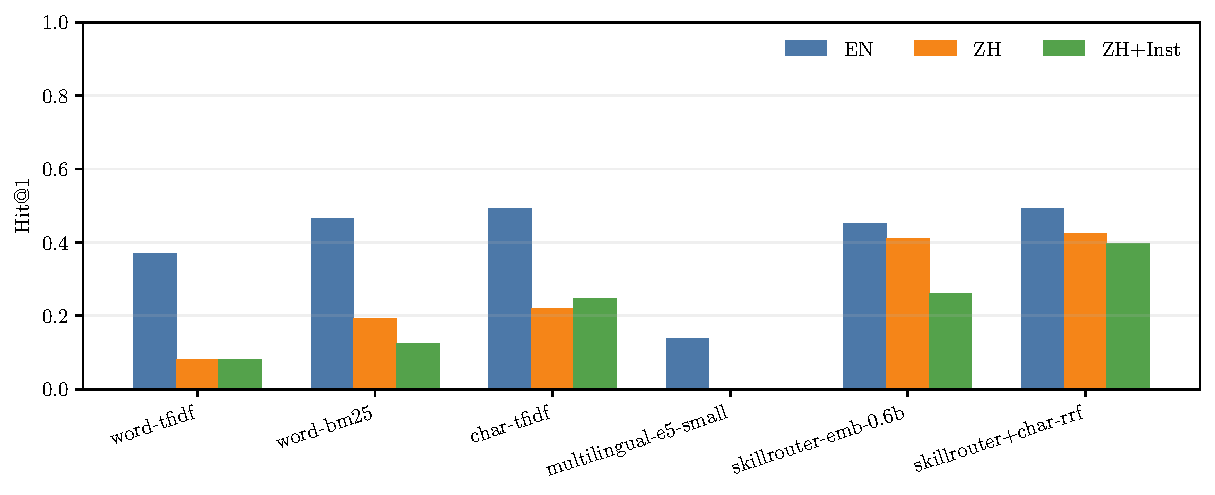
\includegraphics[width=\columnwidth]{figures/skillrouter-hit1.pdf}
  \caption{Hit@1 by query condition on the SkillRouter hard tier.  ZH+Inst is
  the audited Chinese task with one fixed bilingual routing instruction.  All
  conditions retrieve the same English metadata and use the original labels.}
  \label{fig:hit1}
\end{figure}

\paragraph{Latency.}
Sparse methods answer in \SparseLatencyRange{} ms per query.  E5 requires
\EfiveLatency{} ms per query after its candidate embeddings are cached.  The
domain encoder requires \SrLatency{} ms and fusion requires \FusionLatency{}
ms.  The cached mE5 and domain matrices occupy 116\,MB and 309\,MB,
respectively.  These measurements are on Apple MPS and should not be
interpreted as server throughput.

\section{Analysis}

\paragraph{Language mismatch is the main sparse failure mode.}
English metadata contains many exact API names and domain terms.  Chinese
translations preserve the task but remove most lexical overlap.  The fixed
instruction restores only a repeated set of English routing terms, not
task-specific evidence.  The domain encoder reduces the translation loss
without translating 79K descriptions, which is useful when registries aggregate
skills from many authors.

\paragraph{Domain adaptation dominates generic multilinguality.}
The generic multilingual-E5 model performs poorly even on English and retrieves
no core gold at rank 1 for Chinese or instruction-prefixed queries.  A sanity check confirms
that it aligns short English and Chinese sentences, so the failure is not a
broken language encoder.  Rather, generic semantic similarity is insufficient
to distinguish tens of thousands of overlapping procedural descriptions.
Skill-routing training produces far stronger transfer even though the released
checkpoint is labeled English.  The generic encoder's most common Chinese
top-1 prediction appears for 12 of 73 tasks; the domain encoder produces 71
distinct top-1 predictions and no candidate appears more than twice.  Against
character TF--IDF, the domain encoder gains 21 Chinese tasks and loses seven,
but its instruction-prefixed comparison is nearly even (14 gains, 13 losses).
RRF then gains 16 instruction-prefixed tasks over the domain encoder while
losing six, showing that lexical evidence can recover task terms when a fixed
bilingual instruction distracts the dense model.

\paragraph{Instruction prefixes are model dependent.}
The fixed prefix leaves word TF--IDF unchanged, hurts BM25 and the domain
encoder, but improves character retrieval and makes fusion much stronger than
the domain encoder alone.  A host therefore cannot assume that an English or
bilingual meta-instruction helps retrieval simply because it helps an
instruction-following model downstream.  Routing prompts and task prompts have
different objectives and should be evaluated separately.

\section{Limitations and Ethical Considerations}

The multilingual variants are generated and audited by language models, not
professional translators.  Although executable constraints and gold labels
are preserved, subtle phrasing errors may remain.  The public benchmark has
only \PublicTaskCount{} evaluated tasks, so confidence intervals are wide and
domain slices are underpowered.  We evaluate metadata only and truncate dense
inputs to 512 tokens; results do not establish the behavior of full-body
retrieval or longer-context encoders.  Some candidate IDs have identical
name--description text; a stable ID tie-break makes evaluation reproducible,
but exact-ID metrics still penalize metadata-indistinguishable duplicates.  We
do not measure end-to-end task success or no-skill abstention.

We use only public SkillRouter data.  Raw private logs, credentials, work
records, leaked source, and identifying author metadata are excluded.  The
released multilingual file contains task text from the source benchmark and
must retain its upstream attribution and license terms.  Automated routing can
activate instructions with filesystem or shell permissions; higher retrieval
accuracy does not remove the need for permission checks and provenance.

\section{Conclusion}

Bilingual skill routing is not only a smaller version of English retrieval.
At 79K scale, multilingual dense embeddings recover skills lost to lexical
translation, while a fixed bilingual instruction is not a reliable substitute
for task-specific evidence.
Future work should jointly optimize cross-lingual retrieval, prompt design,
full-text routing, and downstream task success.

\label{lastcontentpage}
\bibliography{references}

\end{document}
